\section{Casos de uso}


%\begin{UseCase}[]{USR-CU03.3}{ELiminar Idioma}{
	%Permite al alumno consultar la información de sus idiomas registrados en el perfil.
}
	%----------------------------------------------------------------
	% Datos generales del CU:
	\UCsection{Atributos}
	\UCitem{Actor(es)}{
		\Titem Candidato. 
	}
	\UCitem[admin]{Prioridad}{ 
		\Titem Media.
	}
	\UCitem[admin]{Complejidad}{
		\Titem Baja
	}
	\UCitem{Precondiciones}{
		\Titem El alumno debe de tener una cuenta en el sistema.
		\Titem Se debe de tener previmante registrado al menos un idioma.
	}
	\UCitem{Destino}{
		\Titem \refElem{USR-IU03.1}
	}
	\UCitem{Reglas de Negocio}{
		\Titem Ninguna.
		
	}
	\UCitem{Viene de}{
		\Titem Caso de uso \refIdElem{USR-CU03}.
	}	
\end{UseCase}

%Trayectoria Principal
\begin{UCtrayectoria}
	\UCpaso [\UCactor] Presiona el botón \IUEliminar{} desde la interfaz \refElem{USR-IU03}.
    \UCpaso [\UCsist] Muestra la interfaz \refElem{USR-IU03.3}.
	\UCpaso [\UCactor] Presiona el botón \IUbutton{Aceptar}.\refTray{A}
	\UCpaso [\UCsist] Agrega al catalogo de idiomas el idioma que se quiere eliminar.
	\UCpaso [\UCsist] Eliminar el registro del idioma en el sistem.
	\UCpaso [\UCsist] Muestra la información actualizada en la interfaz \refElem{USR-IU03}.
\end{UCtrayectoria}

\begin{UCtrayectoriaA}[Fin del caso de uso]{A}{El actor desea cancelar el registro}
	\UCpaso [\UCsist] Presiona el botón \IUbutton{Cancelar}.
	\extendUC{USR-CU03}.
\end{UCtrayectoriaA} 


%\begin{UseCase}[]{USR-CU03.3}{ELiminar Idioma}{
	%Permite al alumno consultar la información de sus idiomas registrados en el perfil.
}
	%----------------------------------------------------------------
	% Datos generales del CU:
	\UCsection{Atributos}
	\UCitem{Actor(es)}{
		\Titem Candidato. 
	}
	\UCitem[admin]{Prioridad}{ 
		\Titem Media.
	}
	\UCitem[admin]{Complejidad}{
		\Titem Baja
	}
	\UCitem{Precondiciones}{
		\Titem El alumno debe de tener una cuenta en el sistema.
		\Titem Se debe de tener previmante registrado al menos un idioma.
	}
	\UCitem{Destino}{
		\Titem \refElem{USR-IU03.1}
	}
	\UCitem{Reglas de Negocio}{
		\Titem Ninguna.
		
	}
	\UCitem{Viene de}{
		\Titem Caso de uso \refIdElem{USR-CU03}.
	}	
\end{UseCase}

%Trayectoria Principal
\begin{UCtrayectoria}
	\UCpaso [\UCactor] Presiona el botón \IUEliminar{} desde la interfaz \refElem{USR-IU03}.
    \UCpaso [\UCsist] Muestra la interfaz \refElem{USR-IU03.3}.
	\UCpaso [\UCactor] Presiona el botón \IUbutton{Aceptar}.\refTray{A}
	\UCpaso [\UCsist] Agrega al catalogo de idiomas el idioma que se quiere eliminar.
	\UCpaso [\UCsist] Eliminar el registro del idioma en el sistem.
	\UCpaso [\UCsist] Muestra la información actualizada en la interfaz \refElem{USR-IU03}.
\end{UCtrayectoria}

\begin{UCtrayectoriaA}[Fin del caso de uso]{A}{El actor desea cancelar el registro}
	\UCpaso [\UCsist] Presiona el botón \IUbutton{Cancelar}.
	\extendUC{USR-CU03}.
\end{UCtrayectoriaA} 


%\clearpage
\subsection{USR-IU02.2 Editar Medios de contacto y redes sociales}

\subsubsection{Objetivo}
En la figura \refElem{USR-IU02.2} se muestra la interfaz correspondiente con la funcionalidad descrita en las
trayectorias del caso de uso \refElem{USR-CU02.2} , la cual permite al actor editar sus medios de contacto como son: correos, teléfonos y redes sociales.

\subsubsection{Comandos}
Los siguientes comandos aparecen en la interfaz descrita anteriormente.
\Titem \IUbutton{Aceptar} : Cuando presiona el botón, actualiza la información .
\Titem \IUbutton{Cancelar} : Cuando presiona el botón, muestra la sección anterior.%\refElem{GRL-IU02-2}.

\IUfig{.9}{CasosdeUso/USR-CU02-2/imagenes/USR-IU02.2.png}{USR-IU02.2}{Editar Medios de contacto y redes sociales}  


\clearpage


Los diagramas de casos de uso son una herramienta usada para representar las transacciones entre un actor y el sistema, las cuales siempre tendrán un valor agregado o un propósito para que el actor las realice.
En estos diagramas se podrán observar los siguientes elementos:

\begin{itemize}
	 \UCpaso Representa al sistema mediante un óvalo.
	\item \UCactor Representa al actor que va a interactuar con el sistema.
	\item Relación $<$- - -$<<extends>>$- - -. Indica que un caso de uso \textbf{puede} ejecutarse a partir de otro.
	\item Relación - - -$<<include>>$- - -$>$. Indica que un caso de uso \textbf{debe} ejecutarse a partir de otro.
\end{itemize}

La conexión entre un actor y un caso de uso es por medio de una línea como se muestra en la figura \ref{fig:acUC}.

\begin{figure}[hbtp!]
	\begin{center}
		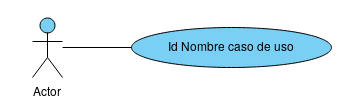
\includegraphics[width=.4\textwidth]{LIT/ActorUC}
	\end{center}
	\label{fig:acUC}
	\caption{Interacción del actor con el caso de uso}
\end{figure}

Los casos de uso se encontrarán dentro de paquetes (representados por carpetas) indicando así que pertenecen a un mismo módulo como se muestra en la figura \ref{fig:pack}.

\begin{figure}[hbtp!]
	\begin{center}
		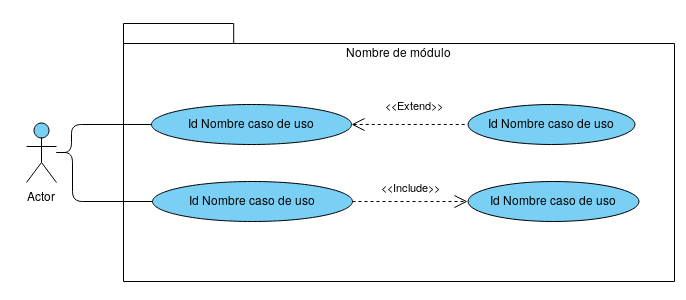
\includegraphics[width=.7\textwidth]{LIT/Paquete}
	\end{center}
	\label{fig:pack}
	\caption{Un Actor con varios caso de uso dentro de un módulo}
\end{figure}

\pagebreak

\subsection{Identificadores de casos de uso}

Los casos de uso se identificarán de acuerdo a la siguiente nomenclatura:

\begin{figure}[hbtp!]
	\begin{center}
		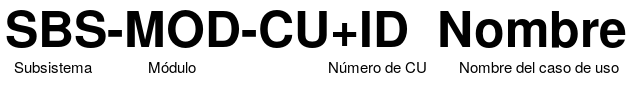
\includegraphics[width=.7\textwidth]{LIT/UCnombre}
	\end{center}
	\label{fig:nomenclatura}
\end{figure}

%\subsection{Modelado de Máquinas de Estados}
  %      \label{sec:ModMaquinas}

%\subsection{Modelado de Actores}
 %       \label{sec:ModActores}
%- - - - - - - - - - - - - - - - - - - - - - - - - - - - -
\subsection{Especificación de casos de uso}

Para poder entender un caso de uso más allá de un diagrama, se lleva a cabo la tarea de especificar cada uno de los casos de uso identificados en el sistema con el fin de describir las secuencias de acciones que realiza el sistema y que lleva a un resultado de valor a un actor específico. Los casos de uso tienen atributos los cuales se describen a continuación:

\begin{description}
	\item[Id] Identificador del caso de uso, el cual debe ser único.
	\item[Nombre] Nombre del caso de uso el cual es descriptivo basándose en la transacción que se realiza.
	\item[Resumen] Es una descripción resumida en la que se especifica la transacción realizada por el caso de uso.
	\item[Actores] Lista de los actores que interactúan con el caso de uso.
	\item[Entradas] Lista los datos de entrada que el caso de uso recibe, los cuales harán referencia al modelo de información.
	\item[Salidas] Lista los datos de salida que el caso de uso genera, por ejemplo: 
	\item[Destino] Indica a dónde se dirigen los datos de salida, por ejemplo: pantalla, impresora, repositorio, hacia un servidor o un archivo.
	\item[Precondiciones] Enlista las cosas que deben haber sucedido para que el caso  de uso se lleve a cabo.
	\item[Postcondiciones] Enlista las cosas que suceden en el sistema o negocio de forma inmediata o a corto plazo una vez que se ejecute el caso de uso.
	\item[Reglas de Negocio] Lista las reglas de negocio que se van a ejecutar en el caso de uso.
	\item[Viene de] Indica cuando el caso de uso se extiende de otro o se incluye en otro.
	\item[Disparador] Aquellas condiciones o motivaciones que el actor tiene para ejecutar el caso de uso.
	\item[Prioridad] Indica el nivel de prioridad que tiene el caso de uso en el sistema. Las opciones son: Muy Alta, Alta, Media, Baja, Muy Baja.
	\item[Transacción primaria] Secuencia de pasos que llevan al caso de uso al éxito.
	\item[Transacciones alternativas] Secuencias de pasos que llevan al caso de uso al éxito o al fracaso.
	\item[Puntos de extensión] Cuando existen casos de uso que pueden ejecutarse a partir del caso de uso en proceso.
\end{description}

\subsection{Diagrama de casos de uso del Sprint 3}
\begin{figure}[hbtp!]
	\begin{center}
		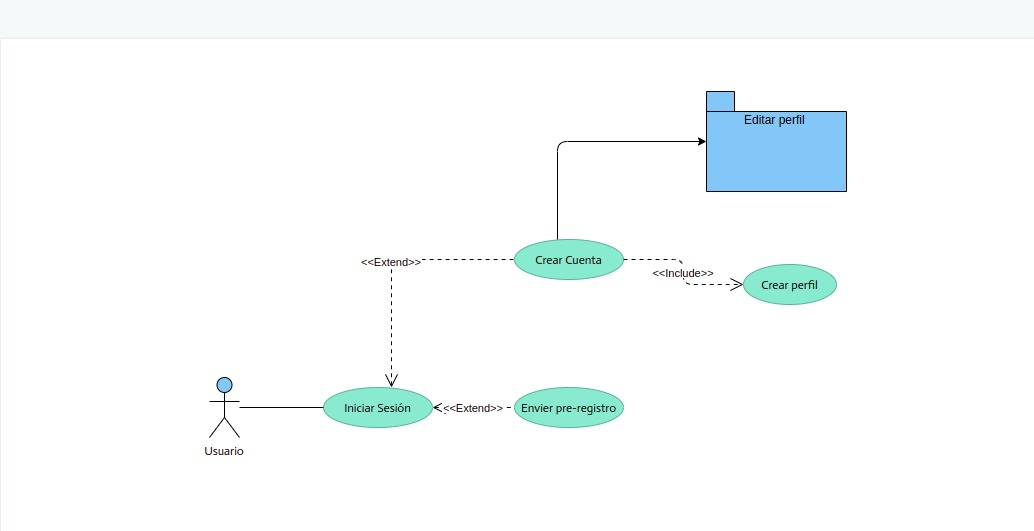
\includegraphics[width=.8\textwidth]{analisisydiseno/imagenes/cuALumno.jpeg}
	\end{center}
	\label{fig:nomenclatura}
\end{figure}

\begin{figure}[hbtp!]
	\begin{center}
		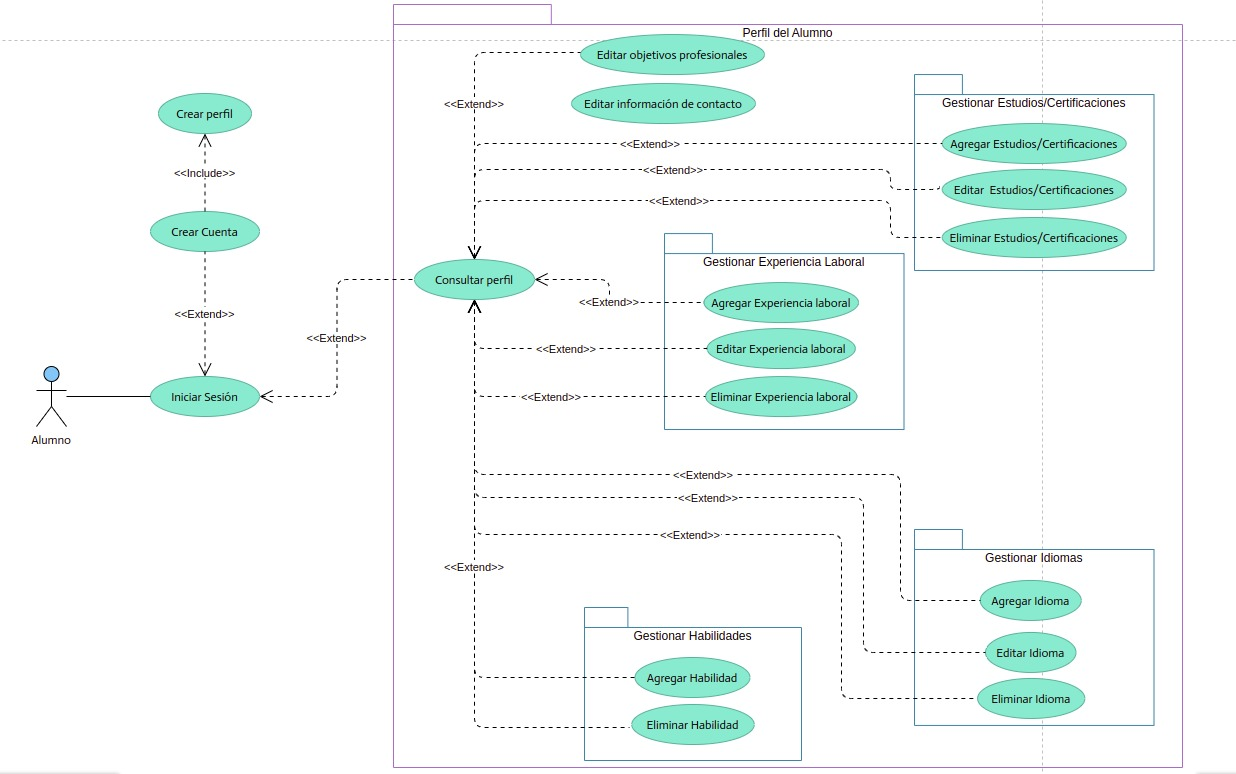
\includegraphics[width=.9\textwidth]{analisisydiseno/imagenes/cu2.jpeg}
	\end{center}
	\label{fig:nomenclatura}
\end{figure}
\clearpage
\subsection{Diagrama de casos de uso del Sprint 4 y 5}
\begin{figure}[hbtp!]
	\begin{center}
		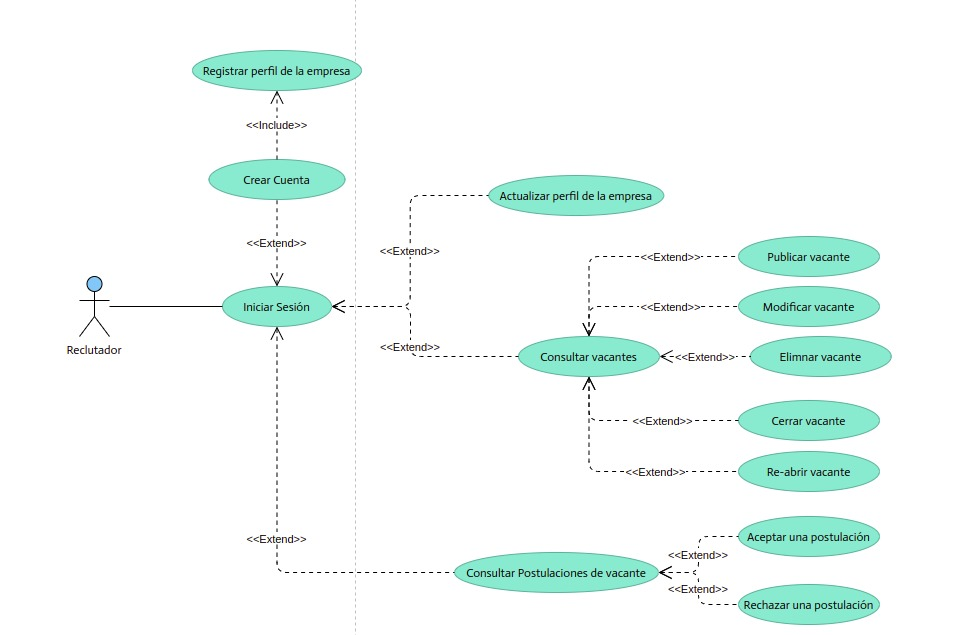
\includegraphics[width=.7\textwidth]{analisisydiseno/imagenes/cu3.jpeg}
	\end{center}
	\label{fig:nomenclatura}
\end{figure}


%---------------------------------------------------------
\section{Modelado de casos de uso}

\subsubsection{Modelo de estados}

Diversas entidades en el sistema  que tienen un comportamiento dinámico en el sistema, 
los que se consideraron en el desarrollo del sistema y ameritaban ser modelados a través de una 
maquina de estados.\\

\subsubsection{Actores del sistema}

 Se definen los actores identificados como participantes en los procesos del sistema. 
 Estos actores son los encargados de llevar a cabo determinadas tareas dentro de cada proceso.\\
 
 \subsubsection{Reglas de negocio}

 Se van describir las reglas de negocio identificadas en el sistema las cuales son una condición que 
 se debe satisfacer cuando se realiza una actividad de negocio.\\
 
\subsubsection{Casos de uso}

Las funcionalidades del sistema son representadas mediante casos de uso. Un caso de uso es una transacción entre un actor y el sistema que tiene un valor agregado o un propósito para que el actor las realice. Los casos de uso se modelan a partir de dos elementos: un diagrama de casos de uso y la
descripción del caso de uso.\\

\subsubsection{Mensajes del sistema}

Los mensajes se refieren a todos aquellos avisos que el sistema muestra al actor para comunicar la ocurrencia de algún evento tal como un error o una operación exitosa. 

